
%% bare_conf.tex
%% V1.4b
%% 2015/08/26
%% by Michael Shell
%% See:
%% http://www.michaelshell.org/
%% for current contact information.
%%
%% This is a skeleton file demonstrating the use of IEEEtran.cls
%% (requires IEEEtran.cls version 1.8b or later) with an IEEE
%% conference paper.
%%
%% Support sites:
%% http://www.michaelshell.org/tex/ieeetran/
%% http://www.ctan.org/pkg/ieeetran
%% and
%% http://www.ieee.org/

%%*************************************************************************
%% Legal Notice:
%% This code is offered as-is without any warranty either expressed or
%% implied; without even the implied warranty of MERCHANTABILITY or
%% FITNESS FOR A PARTICULAR PURPOSE! 
%% User assumes all risk.
%% In no event shall the IEEE or any contributor to this code be liable for
%% any damages or losses, including, but not limited to, incidental,
%% consequential, or any other damages, resulting from the use or misuse
%% of any information contained here.
%%
%% All comments are the opinions of their respective authors and are not
%% necessarily endorsed by the IEEE.
%%
%% This work is distributed under the LaTeX Project Public License (LPPL)
%% ( http://www.latex-project.org/ ) version 1.3, and may be freely used,
%% distributed and modified. A copy of the LPPL, version 1.3, is included
%% in the base LaTeX documentation of all distributions of LaTeX released
%% 2003/12/01 or later.
%% Retain all contribution notices and credits.
%% ** Modified files should be clearly indicated as such, including  **
%% ** renaming them and changing author support contact information. **
%%*************************************************************************


% *** Authors should verify (and, if needed, correct) their LaTeX system  ***
% *** with the testflow diagnostic prior to trusting their LaTeX platform ***
% *** with production work. The IEEE's font choices and paper sizes can   ***
% *** trigger bugs that do not appear when using other class files.       ***                          ***
% The testflow support page is at:
% http://www.michaelshell.org/tex/testflow/



\documentclass[conference]{IEEEtran}
% Some Computer Society conferences also require the compsoc mode option,
% but others use the standard conference format.
%
% If IEEEtran.cls has not been installed into the LaTeX system files,
% manually specify the path to it like:
% \documentclass[conference]{../sty/IEEEtran}





% Some very useful LaTeX packages include:
% (uncomment the ones you want to load)


% *** MISC UTILITY PACKAGES ***
%
%\usepackage{ifpdf}
% Heiko Oberdiek's ifpdf.sty is very useful if you need conditional
% compilation based on whether the output is pdf or dvi.
% usage:
% \ifpdf
%   % pdf code
% \else
%   % dvi code
% \fi
% The latest version of ifpdf.sty can be obtained from:
% http://www.ctan.org/pkg/ifpdf
% Also, note that IEEEtran.cls V1.7 and later provides a builtin
% \ifCLASSINFOpdf conditional that works the same way.
% When switching from latex to pdflatex and vice-versa, the compiler may
% have to be run twice to clear warning/error messages.






% *** CITATION PACKAGES ***
%
%\usepackage{cite}
% cite.sty was written by Donald Arseneau
% V1.6 and later of IEEEtran pre-defines the format of the cite.sty package
% \cite{} output to follow that of the IEEE. Loading the cite package will
% result in citation numbers being automatically sorted and properly
% "compressed/ranged". e.g., [1], [9], [2], [7], [5], [6] without using
% cite.sty will become [1], [2], [5]--[7], [9] using cite.sty. cite.sty's
% \cite will automatically add leading space, if needed. Use cite.sty's
% noadjust option (cite.sty V3.8 and later) if you want to turn this off
% such as if a citation ever needs to be enclosed in parenthesis.
% cite.sty is already installed on most LaTeX systems. Be sure and use
% version 5.0 (2009-03-20) and later if using hyperref.sty.
% The latest version can be obtained at:
% http://www.ctan.org/pkg/cite
% The documentation is contained in the cite.sty file itself.






% *** GRAPHICS RELATED PACKAGES ***
%
\ifCLASSINFOpdf
  % \usepackage[pdftex]{graphicx}
  % declare the path(s) where your graphic files are
  % \graphicspath{{../pdf/}{../jpeg/}}
  % and their extensions so you won't have to specify these with
  % every instance of \includegraphics
  % \DeclareGraphicsExtensions{.pdf,.jpeg,.png}
\else
  % or other class option (dvipsone, dvipdf, if not using dvips). graphicx
  % will default to the driver specified in the system graphics.cfg if no
  % driver is specified.
  % \usepackage[dvips]{graphicx}
  % declare the path(s) where your graphic files are
  % \graphicspath{{../eps/}}
  % and their extensions so you won't have to specify these with
  % every instance of \includegraphics
  % \DeclareGraphicsExtensions{.eps}
\fi
% graphicx was written by David Carlisle and Sebastian Rahtz. It is
% required if you want graphics, photos, etc. graphicx.sty is already
% installed on most LaTeX systems. The latest version and documentation
% can be obtained at: 
% http://www.ctan.org/pkg/graphicx
% Another good source of documentation is "Using Imported Graphics in
% LaTeX2e" by Keith Reckdahl which can be found at:
% http://www.ctan.org/pkg/epslatex
%
% latex, and pdflatex in dvi mode, support graphics in encapsulated
% postscript (.eps) format. pdflatex in pdf mode supports graphics
% in .pdf, .jpeg, .png and .mps (metapost) formats. Users should ensure
% that all non-photo figures use a vector format (.eps, .pdf, .mps) and
% not a bitmapped formats (.jpeg, .png). The IEEE frowns on bitmapped formats
% which can result in "jaggedy"/blurry rendering of lines and letters as
% well as large increases in file sizes.
%
% You can find documentation about the pdfTeX application at:
% http://www.tug.org/applications/pdftex





% *** MATH PACKAGES ***
%
\usepackage{amsmath}
% A popular package from the American Mathematical Society that provides
% many useful and powerful commands for dealing with mathematics.
%
% Note that the amsmath package sets \interdisplaylinepenalty to 10000
% thus preventing page breaks from occurring within multiline equations. Use:
%\interdisplaylinepenalty=2500
% after loading amsmath to restore such page breaks as IEEEtran.cls normally
% does. amsmath.sty is already installed on most LaTeX systems. The latest
% version and documentation can be obtained at:
% http://www.ctan.org/pkg/amsmath





% *** SPECIALIZED LIST PACKAGES ***
%
%\usepackage{algorithmic}
% algorithmic.sty was written by Peter Williams and Rogerio Brito.
% This package provides an algorithmic environment fo describing algorithms.
% You can use the algorithmic environment in-text or within a figure
% environment to provide for a floating algorithm. Do NOT use the algorithm
% floating environment provided by algorithm.sty (by the same authors) or
% algorithm2e.sty (by Christophe Fiorio) as the IEEE does not use dedicated
% algorithm float types and packages that provide these will not provide
% correct IEEE style captions. The latest version and documentation of
% algorithmic.sty can be obtained at:
% http://www.ctan.org/pkg/algorithms
% Also of interest may be the (relatively newer and more customizable)
% algorithmicx.sty package by Szasz Janos:
% http://www.ctan.org/pkg/algorithmicx




% *** ALIGNMENT PACKAGES ***
%
%\usepackage{array}
% Frank Mittelbach's and David Carlisle's array.sty patches and improves
% the standard LaTeX2e array and tabular environments to provide better
% appearance and additional user controls. As the default LaTeX2e table
% generation code is lacking to the point of almost being broken with
% respect to the quality of the end results, all users are strongly
% advised to use an enhanced (at the very least that provided by array.sty)
% set of table tools. array.sty is already installed on most systems. The
% latest version and documentation can be obtained at:
% http://www.ctan.org/pkg/array


% IEEEtran contains the IEEEeqnarray family of commands that can be used to
% generate multiline equations as well as matrices, tables, etc., of high
% quality.




% *** SUBFIGURE PACKAGES ***
\ifCLASSOPTIONcompsoc/
\usepackage[caption=false,font=normalsize,labelfont=sf,textfont=sf]{subfig}
\else
\usepackage[caption=false,font=footnotesize]{subfig}
\fi
\usepackage[export]{adjustbox}
\usepackage{listings}
\usepackage{xparse}
\NewDocumentCommand{\codeword}{v}{%
\texttt{{#1}}%
}
\lstset{language=C,keywordstyle={\bfseries \color{blue}}}
% subfig.sty, written by Steven Douglas Cochran, is the modern replacement
% for subfigure.sty, the latter of which is no longer maintained and is
% incompatible with some LaTeX packages including fixltx2e. However,
% subfig.sty requires and automatically loads Axel Sommerfeldt's caption.sty
% which will override IEEEtran.cls' handling of captions and this will result
% in non-IEEE style figure/table captions. To prevent this problem, be sure
% and invoke subfig.sty's "caption=false" package option (available since
% subfig.sty version 1.3, 2005/06/28) as this is will preserve IEEEtran.cls
% handling of captions.
% Note that the Computer Society format requires a larger sans serif font
% than the serif footnote size font used in traditional IEEE formatting
% and thus the need to invoke different subfig.sty package options depending
% on whether compsoc mode has been enabled.
%
% The latest version and documentation of subfig.sty can be obtained at:
% http://www.ctan.org/pkg/subfig




% *** FLOAT PACKAGES ***
%
%\usepackage{fixltx2e}
% fixltx2e, the successor to the earlier fix2col.sty, was written by
% Frank Mittelbach and David Carlisle. This package corrects a few problems
% in the LaTeX2e kernel, the most notable of which is that in current
% LaTeX2e releases, the ordering of single and double column floats is not
% guaranteed to be preserved. Thus, an unpatched LaTeX2e can allow a
% single column figure to be placed prior to an earlier double column
% figure.
% Be aware that LaTeX2e kernels dated 2015 and later have fixltx2e.sty's
% corrections already built into the system in which case a warning will
% be issued if an attempt is made to load fixltx2e.sty as it is no longer
% needed.
% The latest version and documentation can be found at:
% http://www.ctan.org/pkg/fixltx2e


%\usepackage{stfloats}
% stfloats.sty was written by Sigitas Tolusis. This package gives LaTeX2e
% the ability to do double column floats at the bottom of the page as well
% as the top. (e.g., "\begin{figure*}[!b]" is not normally possible in
% LaTeX2e). It also provides a command:
%\fnbelowfloat
% to enable the placement of footnotes below bottom floats (the standard
% LaTeX2e kernel puts them above bottom floats). This is an invasive package
% which rewrites many portions of the LaTeX2e float routines. It may not work
% with other packages that modify the LaTeX2e float routines. The latest
% version and documentation can be obtained at:
% http://www.ctan.org/pkg/stfloats
% Do not use the stfloats baselinefloat ability as the IEEE does not allow
% \baselineskip to stretch. Authors submitting work to the IEEE should note
% that the IEEE rarely uses double column equations and that authors should try
% to avoid such use. Do not be tempted to use the cuted.sty or midfloat.sty
% packages (also by Sigitas Tolusis) as the IEEE does not format its papers in
% such ways.
% Do not attempt to use stfloats with fixltx2e as they are incompatible.
% Instead, use Morten Hogholm'a dblfloatfix which combines the features
% of both fixltx2e and stfloats:
%
% \usepackage{dblfloatfix}
% The latest version can be found at:
% http://www.ctan.org/pkg/dblfloatfix




% *** PDF, URL AND HYPERLINK PACKAGES ***
%
%\usepackage{url}
% url.sty was written by Donald Arseneau. It provides better support for
% handling and breaking URLs. url.sty is already installed on most LaTeX
% systems. The latest version and documentation can be obtained at:
% http://www.ctan.org/pkg/url
% Basically, \url{my_url_here}.




% *** Do not adjust lengths that control margins, column widths, etc. ***
% *** Do not use packages that alter fonts (such as pslatex).         ***
% There should be no need to do such things with IEEEtran.cls V1.6 and later.
% (Unless specifically asked to do so by the journal or conference you plan
% to submit to, of course. )


% correct bad hyphenation here
\hyphenation{op-tical net-works semi-conduc-tor}


\begin{document}
%
% paper title
% Titles are generally capitalized except for words such as a, an, and, as,
% at, but, by, for, in, nor, of, on, or, the, to and up, which are usually
% not capitalized unless they are the first or last word of the title.
% Linebreaks \\ can be used within to get better formatting as desired.
% Do not put math or special symbols in the title.
\title{Project 2: Face Swap}


% author names and affiliations
% use a multiple column layout for up to three different
% affiliations
\author{\IEEEauthorblockN{Radha Saraf}
\IEEEauthorblockA{Email: rrsaraf@wpi.edu}
\and
\IEEEauthorblockN{Sai Ramana Kiran Pinnama Raju}
\IEEEauthorblockA{Email: spinnamaraju@wpi.edu\\
Using 1 late day}
}
% conference papers do not typically use \thanks and this command
% is locked out in conference mode. If really needed, such as for
% the acknowledgment of grants, issue a \IEEEoverridecommandlockouts
% after \documentclass

% for over three affiliations, or if they all won't fit within the width
% of the page, use this alternative format:
% 
%\author{\IEEEauthorblockN{Michael Shell\IEEEauthorrefmark{1},
%Homer Simpson\IEEEauthorrefmark{2},
%James Kirk\IEEEauthorrefmark{3}, 
%Montgomery Scott\IEEEauthorrefmark{3} and
%Eldon Tyrell\IEEEauthorrefmark{4}}
%\IEEEauthorblockA{\IEEEauthorrefmark{1}School of Electrical and Computer Engineering\\
%Georgia Institute of Technology,
%Atlanta, Georgia 30332--0250\\ Email: see http://www.michaelshell.org/contact.html}
%\IEEEauthorblockA{\IEEEauthorrefmark{2}Twentieth Century Fox, Springfield, USA\\
%Email: homer@thesimpsons.com}
%\IEEEauthorblockA{\IEEEauthorrefmark{3}Starfleet Academy, San Francisco, California 96678-2391\\
%Telephone: (800) 555--1212, Fax: (888) 555--1212}
%\IEEEauthorblockA{\IEEEauthorrefmark{4}Tyrell Inc., 123 Replicant Street, Los Angeles, California 90210--4321}}




% use for special paper notices
%\IEEEspecialpapernotice{(Invited Paper)}




% make the title area
\maketitle

% As a general rule, do not put math, special symbols or citations
% in the abstract
% \begin{abstract}
% The abstract goes here.
% \end{abstract}

% no keywords




% For peer review papers, you can put extra information on the cover
% page as needed:
% \ifCLASSOPTIONpeerreview
% \begin{center} \bfseries EDICS Category: 3-BBND \end{center}
% \fi
%
% For peerreview papers, this IEEEtran command inserts a page break and
% creates the second title. It will be ignored for other modes.
\IEEEpeerreviewmaketitle

\begin{abstract}
The aim of this project is to implement an end-to-end pipeline to swap faces in a video. We explore both classical and deep learning methods to this end. 
\end{abstract}

Irrespective of the method however, the strategy or the pipeline in both the cases remain same and is shown in the figure \ref{fig:face_swap_pipeline}


\begin{figure}[!h]
    \centering
    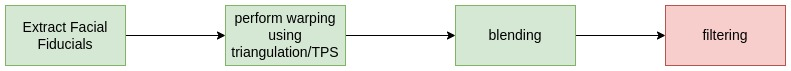
\includegraphics[width=0.5\textwidth]{media/face_swap_pipeline.jpg}
    \caption{Face swap pipeline}
    \label{fig:face_swap_pipeline}
\end{figure}

\section{Phase I: Classical Approach}
One of the main challenges in face swapping is to find a function to ``map'' each pixel in one face to each pixel in the other face. For this mapping we first find a set of landmarks and their correspondences in the target faces. We used \codeword{dlib} library for the same and obtained facial fiducials as shown in the figure \ref{fig:dlib_landmarks}

After obtaining the fiducials, our next step is to perform the mapping. A naive approach for this wouldve been is to map pixel by pixel in 3D space. This approach although simple, wouldve given us pretty good results. However, this approach is computationally intensive and wouldnt work well in real time applications. Hence, we simplify this problem of computationally complexity by approximating the facial structure in 2D space. We achieve this using the following 2 methods,
\begin{enumerate}
    \item Delaunay Triangulation
    \item Thin Plate Splines \cite{tps}
\end{enumerate}


\subsection{Face swapping using delaunay triangulation}
The strategy for delaunay triangulation is as follows, 
\begin{enumerate}
    \item take landmarks obtained in the previous step
    \item construct triangles using the landmarks
    \item construct a convex hull around the face
    \item inverse warp each pixel within triangle using barycentric coords and affine transformation
    \item warp the faces
\end{enumerate}



Following subsequent subsections discuss on some of the observations, challenges and finally results of this approach in the swapping faces
\subsubsection{Inconsistent Landmarks}
One of the initial challenge we faced during this was that some of the landmarks obtained from the above library are not unique. Some of the points are representing the same points, because of which there were some problems in the pipeline downstream. A simple problem was that there were singular matrices while finding barycentric coordinates. To avoid this issue we ran a unique check after the fiducials are obtained 

\begin{figure}[]
\centering
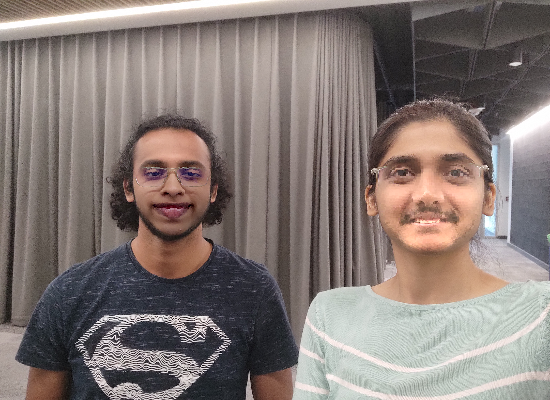
\includegraphics[width=0.4\textwidth]{media/blend_after.png}
\caption{Output image after blending using TPS}
\label{fig:after_blending}
\end{figure}

\begin{figure}[]
    \centering
    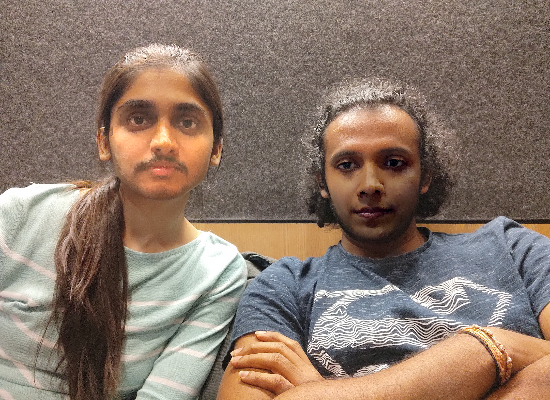
\includegraphics[width=0.4\textwidth]{media/correct_triangulation.png}
    \caption{Face Swap using Triangluation after accouting for the numerical inaccuracies in the inverse calculation }
    \label{fig:barycentric_solution}
\end{figure}

\subsubsection{Finding triangle correspondences}
In order to construct the triangulation using the landmarks we use the dual of Voronoi diagram. Vornoi diagram of our team can be seen in the figure \ref{fig:voronoi_test}. One can easily identify that dissimilar voronoi diagrams by paying attention to the number of ``horns'' in the voronoi output. Theoretically, for similar faces, we could obtain the approximately same voronoi diagram and hence same triangulation using this formulation. However, in reality faces are hardly similar. 


\begin{figure}[]
    \centering
    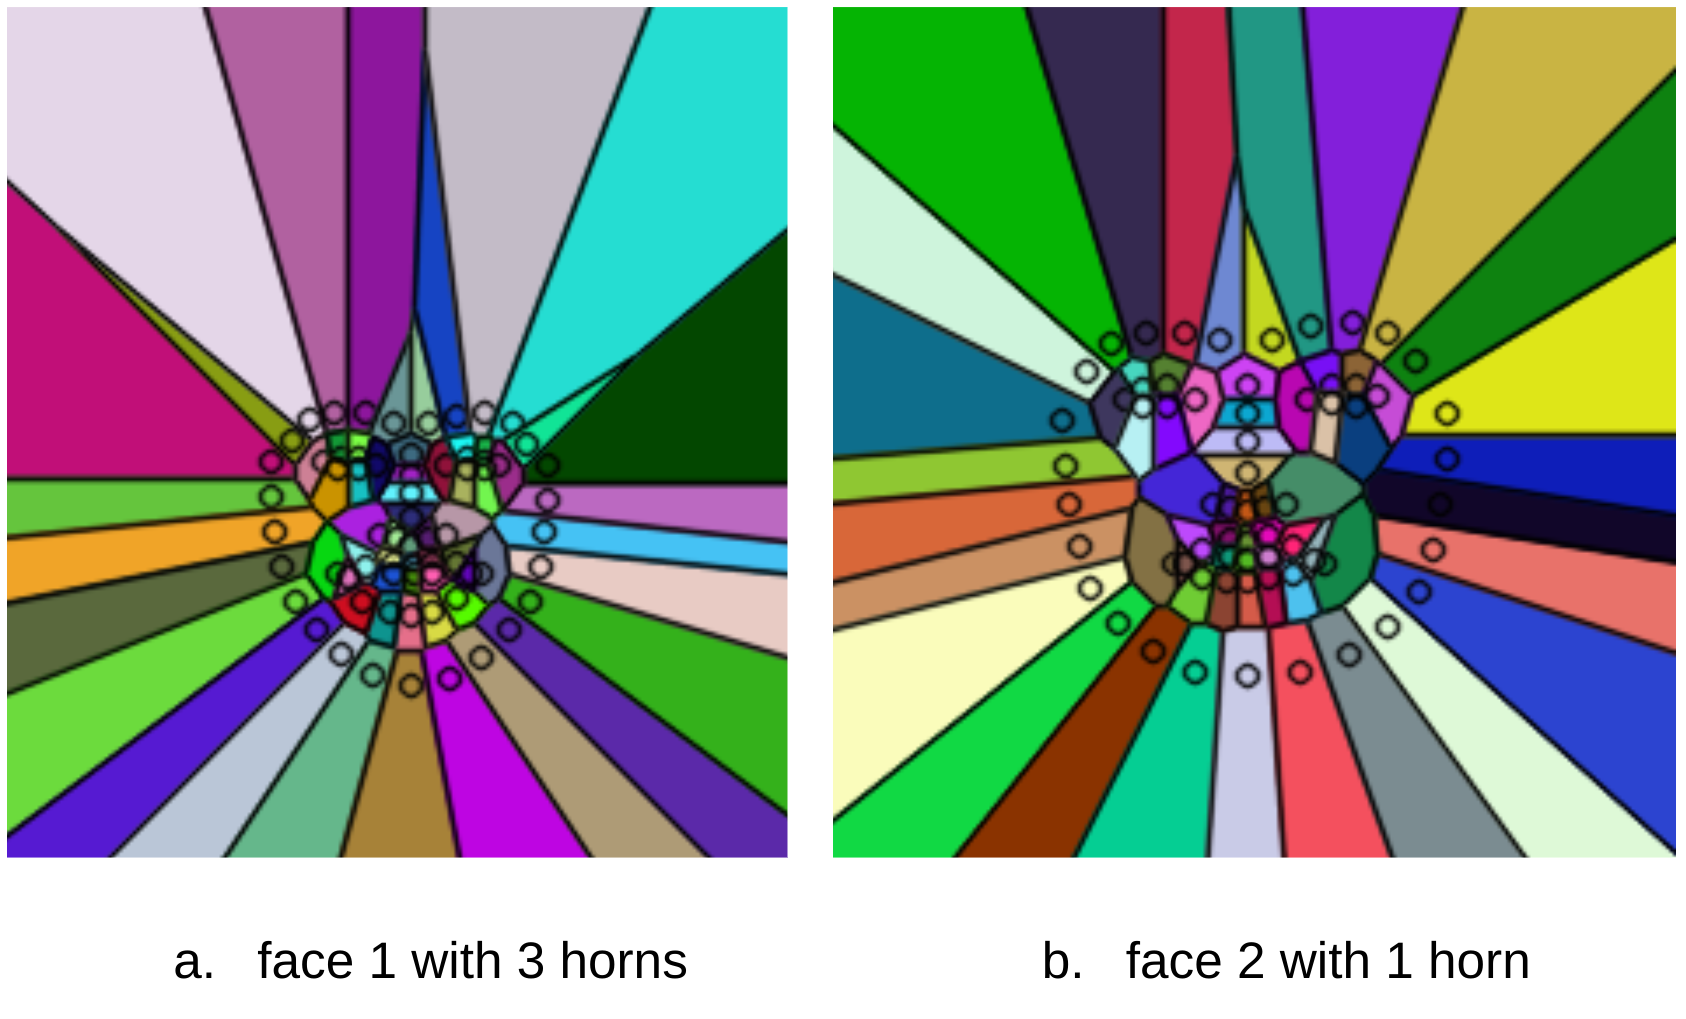
\includegraphics[width=0.4\textwidth]{media/voronoi_merge.png}
    \caption{Voronoi diagram due to dissimilar faces}
    \label{fig:voronoi_test}
\end{figure}



\begin{figure}[!htbp]
\centering
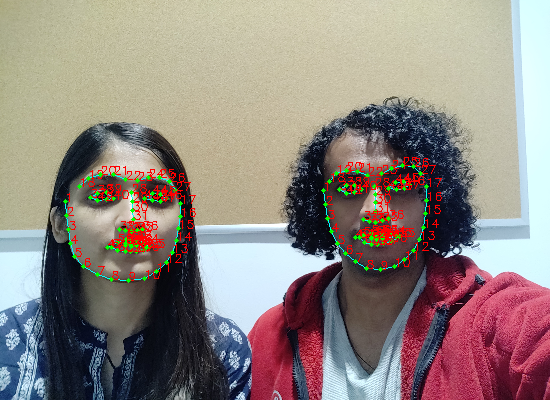
\includegraphics[width=0.4\textwidth]{media/landmarks.png}
\caption{Face Fiducials}
\label{fig:dlib_landmarks}
\end{figure}

To further simplify this, we first obtained the triangulation on one face patch and applied the same triangulation on the other face patch using the landmark correspondences. Essentially, since we know the landmark correspondences we \textit{forced} the triangle correspondences across the faces using one as a reference. Figure \ref{fig:triangulation_correct} shows the triangulation obtained on both the faces. The colors, order and structure of the triangles across the face patches are identical in this version. 

\begin{figure}[]
    \centering
    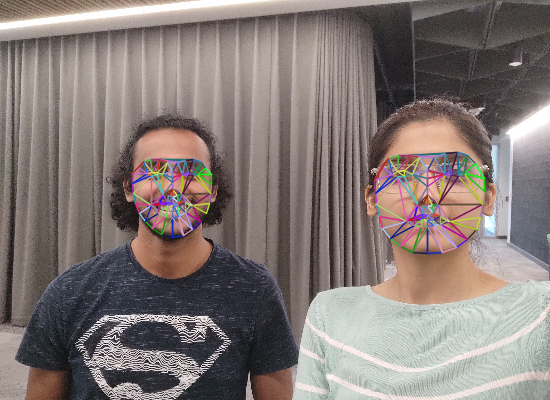
\includegraphics[width=0.4\textwidth]{media/triangulation_solution.png}
    \caption{Correct Triangulation by force}
    \label{fig:triangulation_correct}
\end{figure}


\subsubsection{Inverse warping and Numerical inaccuracies}
Once we have the triangle correspondences between the faces, we just need to apply the affine transformation from source image to the destination image giving us a \textit{forward warp} of the patch. However, this approach has following 2 issues 
\begin{enumerate}
    \item Holes in the destination image
    \item destination pixels might be subpixel values instead of pixel indices
\end{enumerate}
We mitigate these 2 issues using inverse warping of the patch. i.e we first construct the destination grid on which we need to \textit{warp to}. Since we have a concrete destination indices we reverse map these indices to the source image and get the pixel values from these coordinates. If they fall on the subpixel values in the source image, we interpolate the values and get these pixels hence mitigating both of the above issues

One of the ways to achieve this inverse warping of the pixels within the triangle is to calculate ``Barycentric Coordinates'' of pixels in the destination image and use these coordinates to find the pixel correspondencies in the source image triangles. These coordinates are essentially factors while representing the point within triangle as a linear combination of the triangle vertex. Hence, for this reason, every barycentric coordinate obtained for a point within a triangle \textbf{must} and will satisfy the conditions mentioned in equations \ref{eq:barycentric_coords}. Once we get this coordinate we can map destination image pixel to source image pixel. 
\begin{equation}\label{eq:barycentric_coords} 
\begin{aligned}
    \alpha \in [0,1] \\
    \beta \in [0,1]\\
    \gamma \in [0,1]\\
    \alpha + \beta + \gamma \in (0,1]
\end{aligned}
\end{equation}

However, following the steps above, resulted in the figure \ref{fig:barycentric_problem}. The figure without blending shows the holes despite the inverse warp on both of the faces. The reason for this is due to the numerical inaccuracies in the inverse calculation of the barycentric coordinate on the destination image. Essentially, these inaccuraccies in the inverse matrix have not been taken into account initially when the mapping was performed giving rise the aforementioned face swap. We later took this into account by adding a small epsilon $1e-6$ to the conditions mentioned in the equations \ref{eq:barycentric_coords} that need to be satisfied by the barycentric coordinates resulting in the figure \ref{fig:barycentric_solution} 
%%% TODO remove blending the following image %%%%
\begin{figure}[]
    \centering
    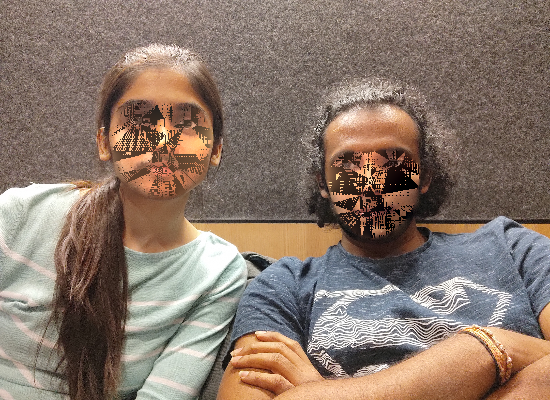
\includegraphics[width=0.4\textwidth]{media/incorrect_triangulation_output.png}
    \caption{Missing Data in triangulation method}
    \label{fig:barycentric_problem}
\end{figure}

\subsubsection{Observations}
This method although simple to understand and implement, has 2 issues 
\begin{itemize}
    \item Artificial texture: the resulting images from this method look planar and seem very artificial in nature. It lacks the texture the original images has.
    \item Speed: This method is amazingly slow and cannot be implemented in real time and definitely not in edge devices. It took around $15$sec to perform face swapping on an intel i7 10 core desktop. This could be because of latencies in python and the method overall
\end{itemize}


\subsection{Face swapping using thin plate splines(TPS)}

Triangulation assumes that we are doing affine transformation on each triangle. This is not the best way to do warping since the human face isn't planar. Some of the triangles are such that the 3 vertices are all in different planes in 3d space. The triangulation for these triangles isn't great and consequently the warping results aren't perfect either. Since the face has a very complex and smooth shape, we use thin plate splines to approximate its variations.

We compute a TPS that maps from the feature points in one face to the corresponding feature points in the other face. Also, we need to do this for two splines, one for the x coordinate and one for the y.

The strategy for warping using TPS is as follows. The workflow assumes we are warping face one to two.
\begin{enumerate}
    \item Obtained fiducial landmarks from dlib for both faces.
    \item Model landmarks in face one as a parametric spline of the landmarks in face two.
    \item Solve for the model and find the parameters.
    \item Use the parameters to warp every point in a rectangle around face one to face two.
    \item Grab a convex hull around the face for better face fit.
    \item Repeat for face two.
\end{enumerate}

The initial result from this vanilla workflow turned out pretty bad as shown in figure \ref{fig: initial_result_tps}. The patch is broken in places probably as a consequence of the incorrect warping.

We thought this was the case because we were warping all the pixels within a rectangle around the face but using only the facial landmarks to get the parameters for warping. So, we included the rectangle corners and the centers of the rectangle sides as additional features in the fiducial landmarks set. This helped. It got us rid of the missing patch as seen in figure \ref{fig: inc_rect_sides_centers}. But it was still nowhere close to perfect.

With everything else in place correctly, the radial basis function was one of the potential reasons why the warping could have gone wrong. We started testing out different ideas here. At first we changed the log function to bases 10 and 2 with not much difference in the result. We used an L2 norm in place of the L1 norm but that also wasn't promising and so we tried changing the function itself and went with the classic gaussian as the first choice. The differences in these RBFs can be seen visually in figure \ref{fig:rbf}. 

The results of changing the RBF to gaussian were quite promising as can be seen in figures \ref{fig:inc_gaussian_rbf_face1} and \ref{fig:inc_gaussian_rbf_face2} for the two faces.

The very evident next step from these results was to make the warping fit to the face since the rectangle looked very unnatural. To overcome this, we found the convex hull of the facial landmarks and created a binary mask from it to only consider the warped points within this mask. As can be seen in figures \ref{fig:inc_convex_hull_both_faces_1} and \ref{fig:inc_convex_hull_both_faces_2}, we get better face fit for the warpings using the convex hull trick.

\subsubsection{Observations}
One of the main observation of TPS compared to triangulation method is that it's fast! Every step of the pipeline is well vectorized and results are easily evident. On the same platform as earlier, it took around $0.5$sec to produce the output. It is still not close to real time but it is sufficiently good to take it forward for optimization and apply it for non critical applications. 

Another observation is that, it is comparatively very smooth and has a nice texture. However, it is still not stable and has a wavy output in the videos. This could be because of the choice of gaussian RBF. Need to experiment with better RBF models 

\begin{figure}[!htbp]
\centering
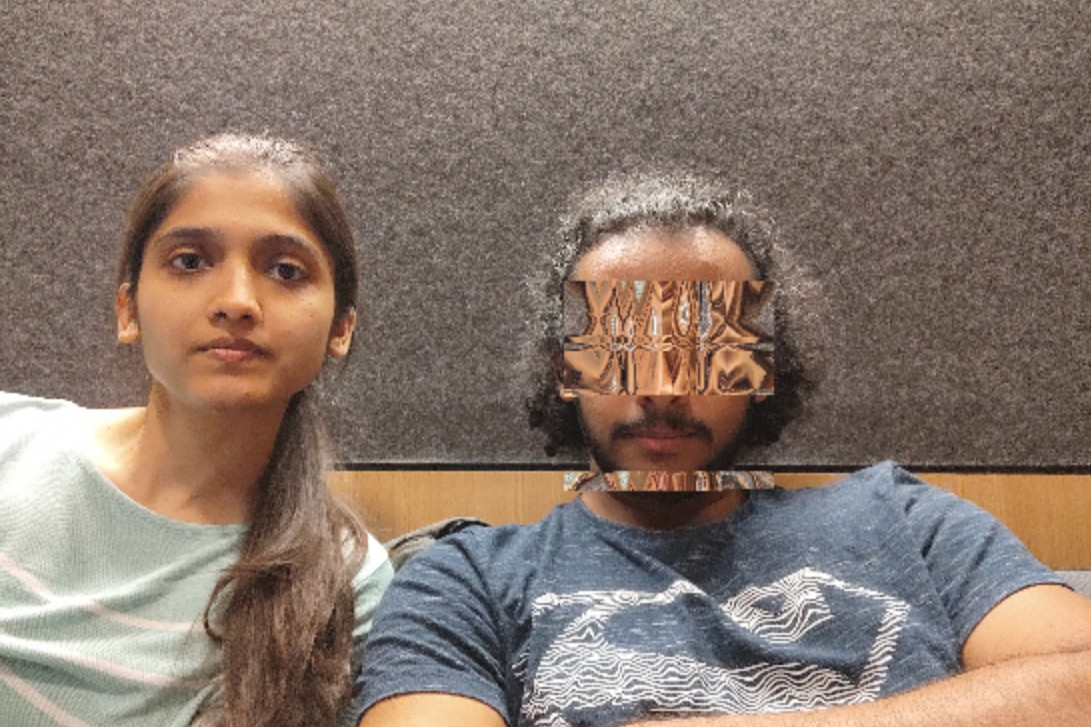
\includegraphics[width=0.4\textwidth]{media/initial_result_tps.jpg}
\caption{Initial results: TPS}
\label{fig: initial_result_tps}
\end{figure}


\begin{figure}[!htbp]
\centering
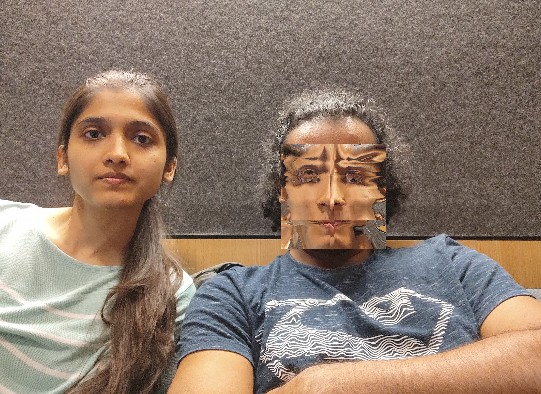
\includegraphics[width=0.4\textwidth]{media/incorporate_rect_sides_centers.jpg}
\caption{On incorporating centers of rect sides}
\label{fig: inc_rect_sides_centers}
\end{figure}

\begin{figure}[!htbp]
\centering
\minipage{0.24\textwidth}
  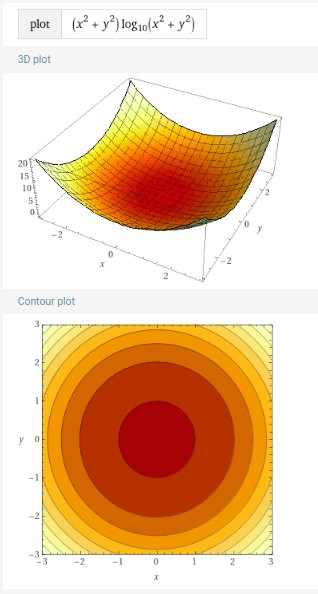
\includegraphics[width=\linewidth]{media/RBF_log.jpg}
\endminipage
\minipage{0.24\textwidth}
  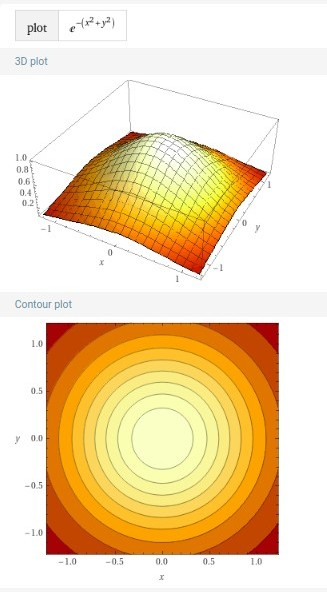
\includegraphics[width=\linewidth]{media/RBF_gaussian.jpg}
\endminipage
\caption{Log and Gaussian as Radial Basis Functions}
\label{fig:rbf}
\end{figure}

\begin{figure}[!htbp]
\centering
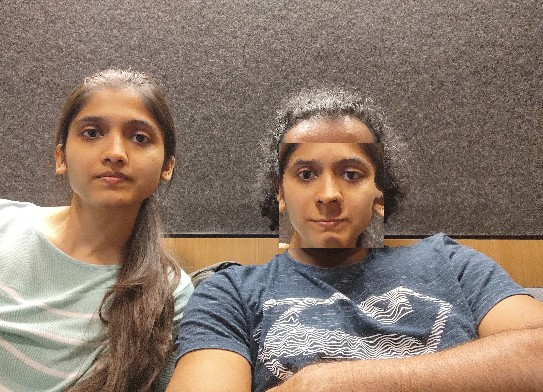
\includegraphics[width=0.4\textwidth]{media/incorporate_gaussian_face1.jpg}
\caption{Gaussian RBF on face 1}
\label{fig:inc_gaussian_rbf_face1}
\end{figure}

\begin{figure}[!htbp]
\centering
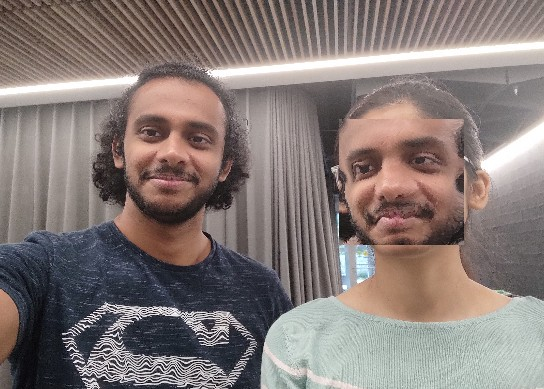
\includegraphics[width=0.4\textwidth]{media/incorporate_gaussian_face2.jpg}
\caption{Gaussian RBF on face 2}
\label{fig:inc_gaussian_rbf_face2}
\end{figure}

\begin{figure}[!htbp]
\centering
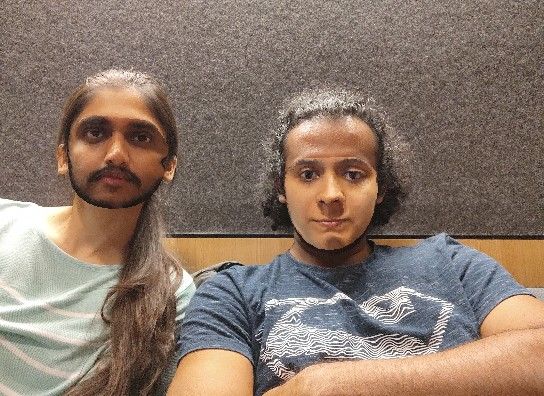
\includegraphics[width=0.4\textwidth]{media/convex_hull_both_faces1.jpg}
\caption{On incorporating convex hull for both faces 1}
\label{fig:inc_convex_hull_both_faces_1}
\end{figure}

\begin{figure}[!htbp]
\centering
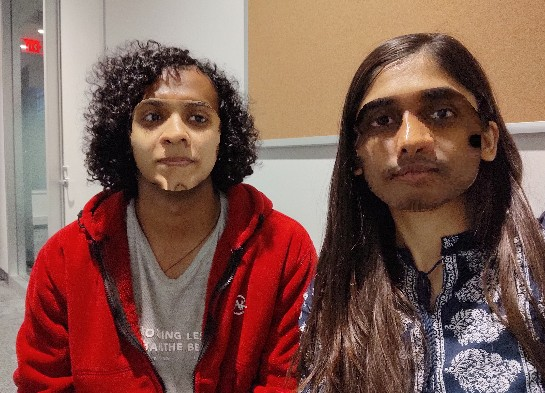
\includegraphics[width=0.4\textwidth]{media/convex_hull_both_faces2.jpg}
\caption{On incorporating convex hull for both faces 2}
\label{fig:inc_convex_hull_both_faces_2}
\end{figure}

\section{Blending}

After swapping the faces, we need to blend the images to make it look more natural to the scene. We used OpenCV's poisson blending available in \codeword{seamlessClone} functionality. To this end, we took a step back and instead of modifying the images directly, we created masks of the images that needs to blended together. Figure \ref{fig:blending_inputs} shows the inputs to the blending operation and \ref{fig:before_blending} shows the actual frame and finally \ref{fig:after_blending} shows the output the frame. 

\begin{figure}[!htbp]
\centering
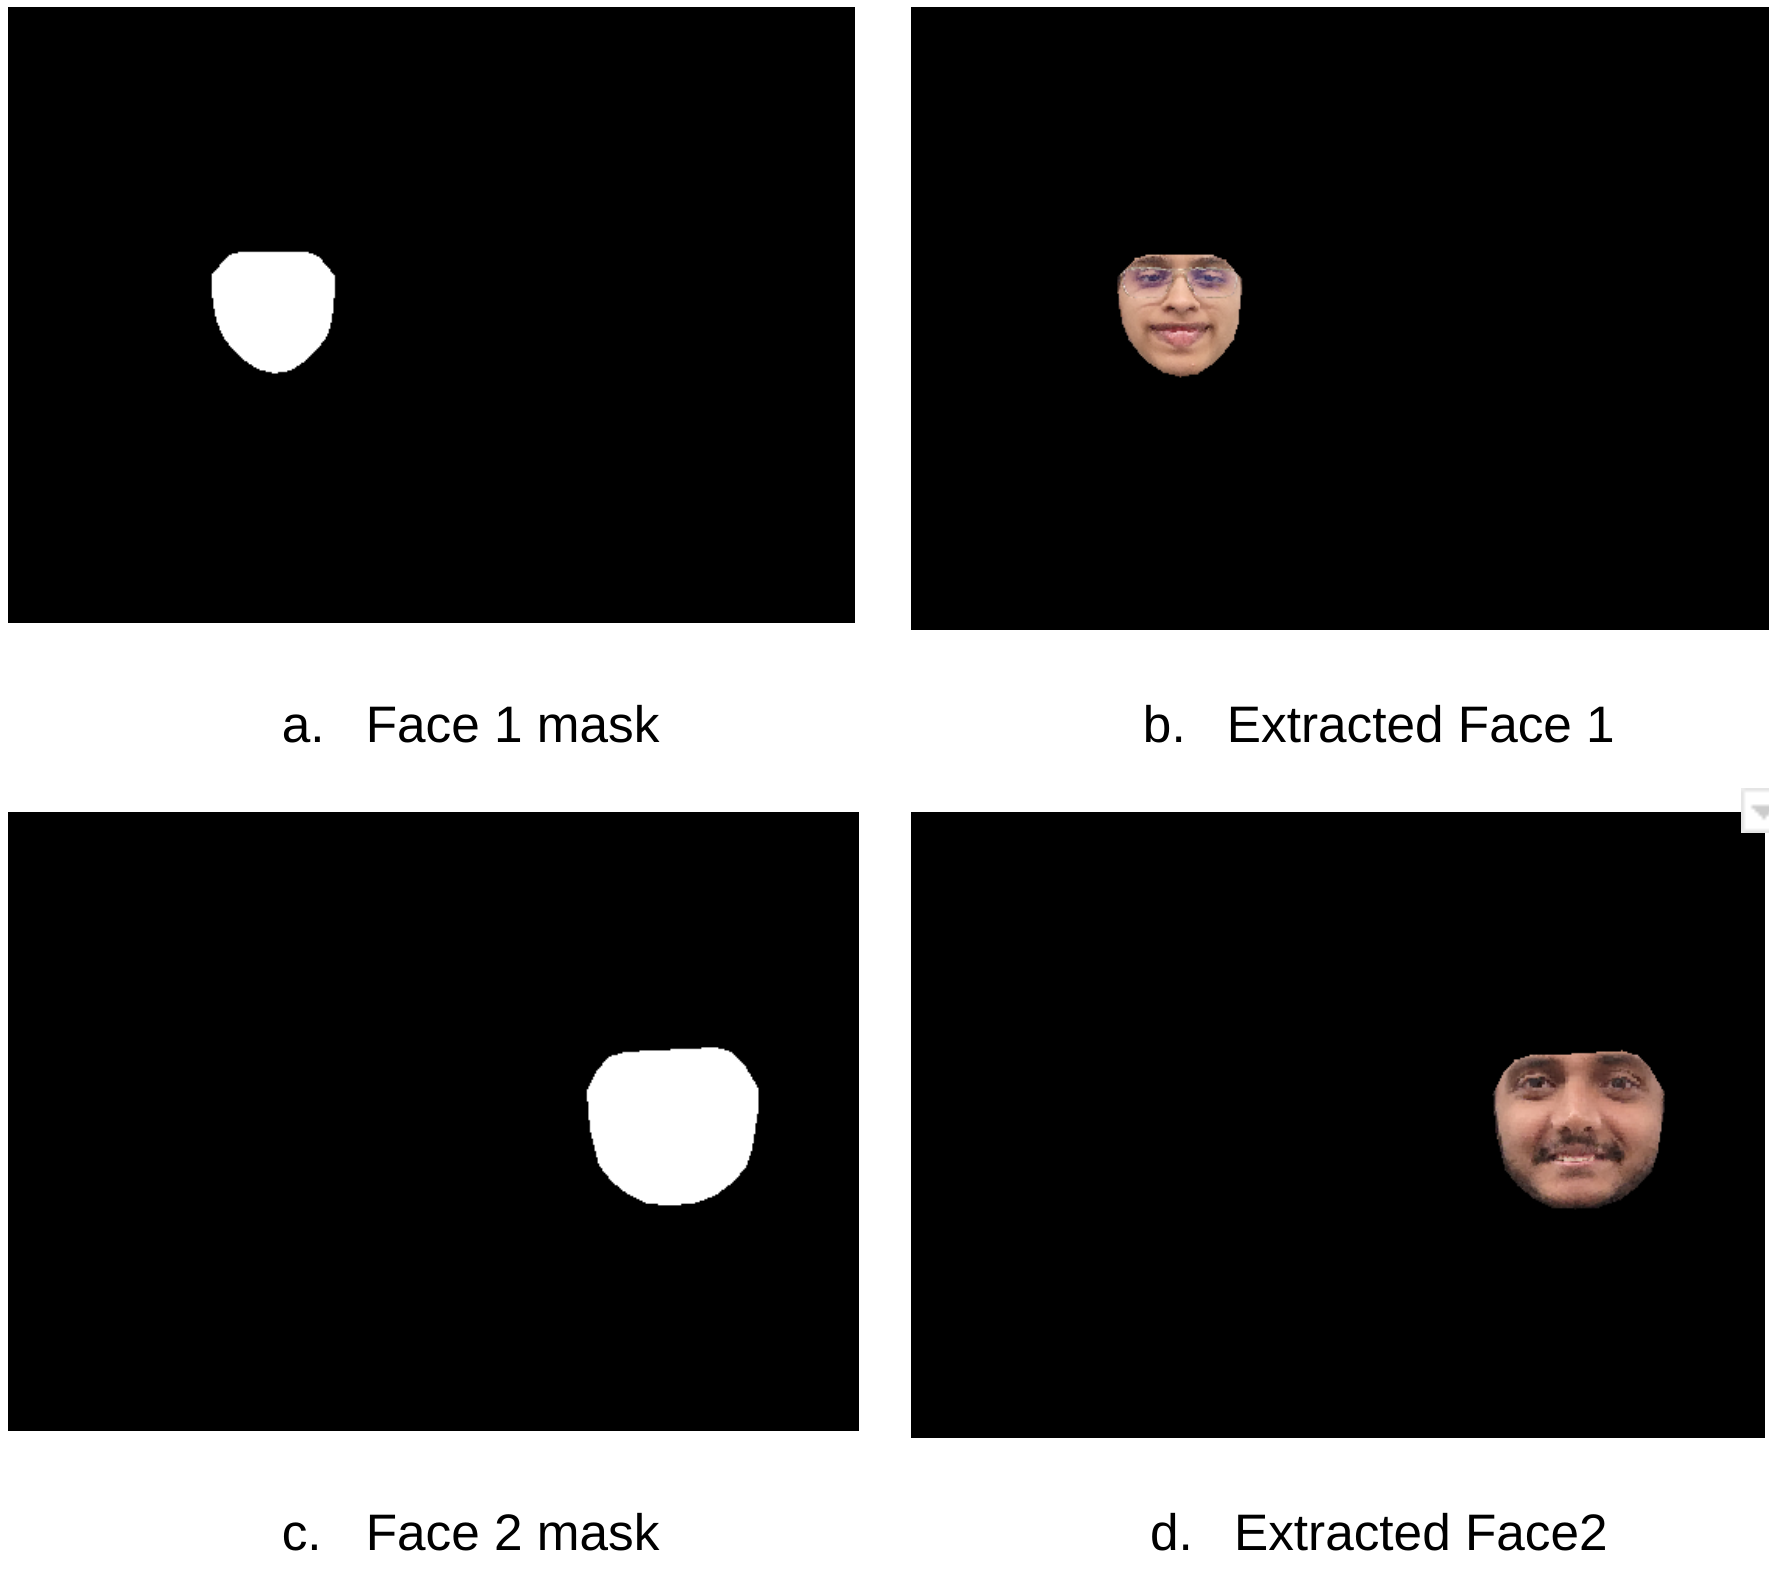
\includegraphics[width=0.4\textwidth]{media/blending_inputs.png}
\caption{Blending Inputs}
\label{fig:blending_inputs}
\end{figure}

\begin{figure}[!htbp]
\centering
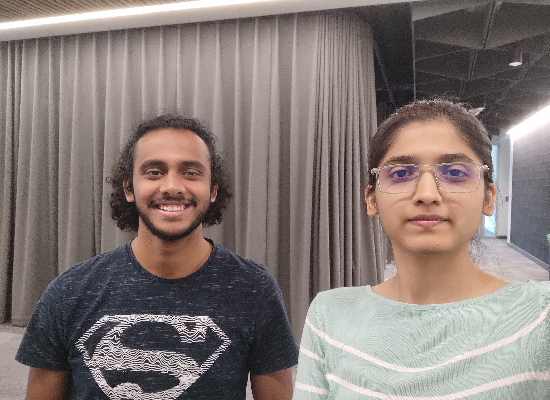
\includegraphics[width=0.4\textwidth]{media/before_blend_before.png}
\caption{Input image before blending}
\label{fig:before_blending}
\end{figure}

\section{Motion Filtering}
We found that bounding box that we get from the dlib library is sometimes inconsistent and ``jerky'' in nature. To make it more smooth we used kalman filter available in OpenCV. Figure \ref{fig:kalman_bounding_box} shows the measurement and predicted bounding boxes by kalman filter. However, results using this were not that different from the earlier results and need to incorporate actualy rectangle relationships for better results


\begin{figure}[]
\centering
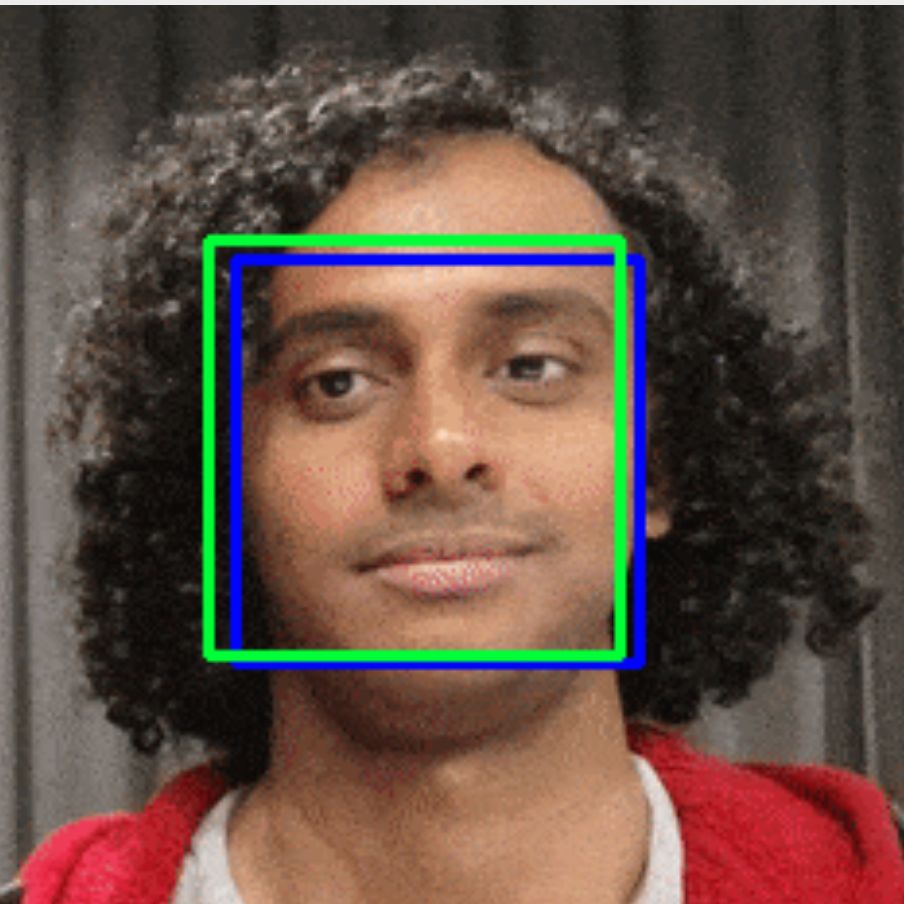
\includegraphics[width=0.4\textwidth]{media/kalman_filter_bb.png}
\caption{Motion Filtering using kalman filtering. Green indicates the predicted motion by the kalman filter Blue indicates actual measurement }
\label{fig:kalman_bounding_box}
\end{figure}


\section{Phase II Deep Learning approach}
In this approach we run the PRNet \cite{deep_learning} to get depth map and fiducials from the video. make use of the fiducials that we get from the PRNet \cite{deep_learning}. Unfortunately, we couldnt setup the code to perform texture swapping using the depth map as the authors of the PRNet says. Hence, we use the fiducials and apply TPS on top of it. The only difference is enhanced fiducials and swapping has same output as the TPS. Figure \ref{fig:dl_output_place_holder}

Another approach to use dense map, is to use techniques such as point cloud to point cloud deformation and comparison. These techniques can be used to swap faces

\begin{figure}[]
\centering
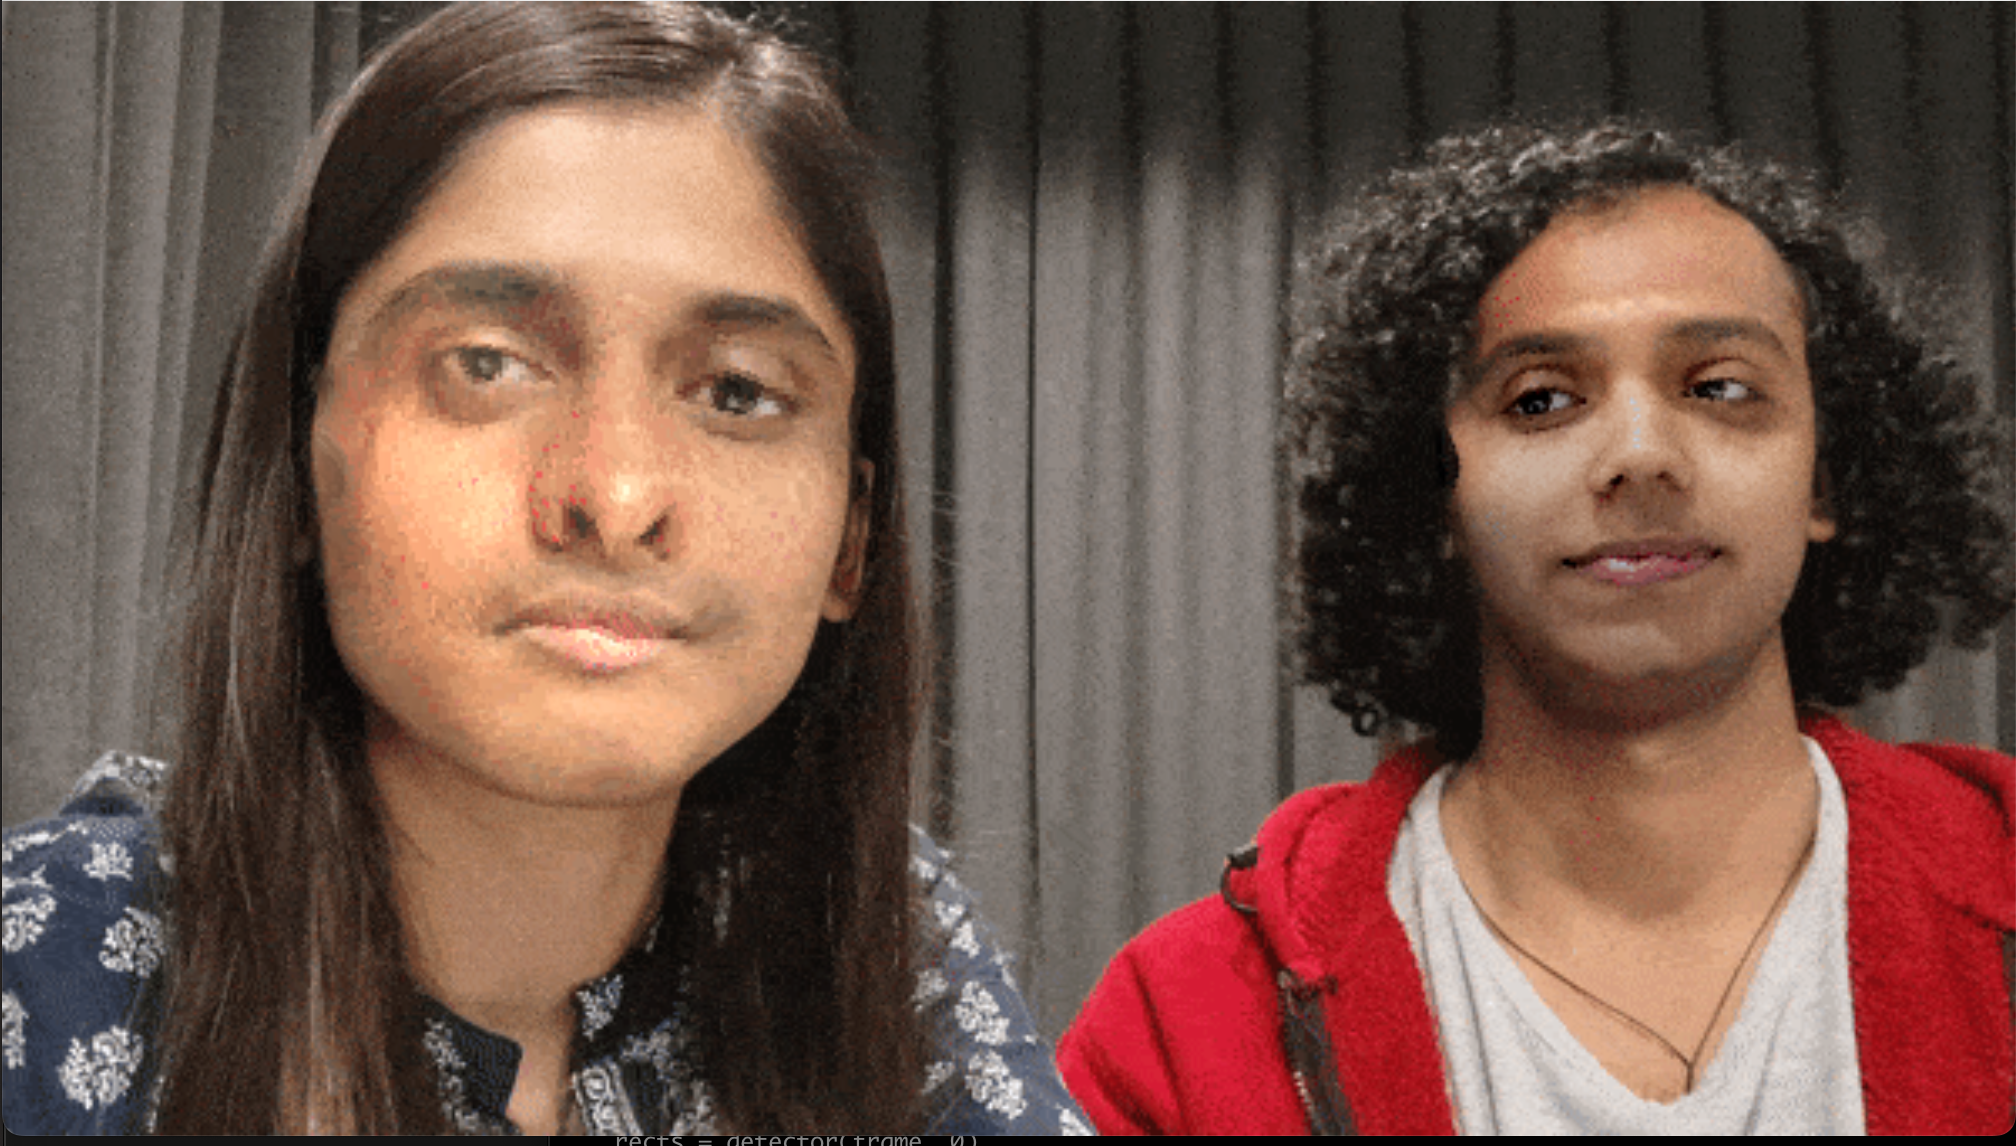
\includegraphics[width=0.4\textwidth]{media/DL_output_ph.png}
\caption{Deep learning output using TPS}
\label{fig:dl_output_place_holder}
\end{figure}


\begin{thebibliography}{00}

\bibitem{tps}F. L. Bookstein, "Principal warps: thin-plate splines and the decomposition of deformations," in IEEE Transactions on Pattern Analysis and Machine Intelligence, vol. 11, no. 6, pp. 567-585, June 1989, doi: 10.1109/34.24792.

\bibitem{deep_learning} Zhu, Xiangyu, Xiaoming Liu, Zhen Lei, and Stan Z. Li. "Face alignment in full pose range: A 3d total solution." IEEE transactions on pattern analysis and machine intelligence 41, no. 1 (2017): 78-92.

\end{thebibliography}




% that's all folks
\end{document}


